%%%%%%%%%%%%% Begin document %%%%%%%%%%%%%
\documentclass[]{article}

%%%%%%%%%%%%% Package imports %%%%%%%%%%%%%
\usepackage[T1]{fontenc}
\usepackage{titlesec}
\usepackage[backend=biber, style=numeric]{biblatex}
\usepackage{multicol}
\usepackage{easyReview}
\usepackage{matlab-prettifier}
\usepackage[letterpaper, margin=1in]{geometry}
\usepackage{amsmath}
\usepackage{amssymb}
\usepackage{graphicx}
\usepackage{bbm}
\usepackage{hyperref}
\usepackage{tikz}
\usetikzlibrary{arrows.meta, calc, decorations.markings, positioning}
%%%%%%%%%%%%% Macro definitions %%%%%%%%%%%%%

\newcommand{\pd}[2]{\frac{\partial\;#1}{\partial\;#2}}
\newcommand{\pddown}[2]{\frac{\partial}{\partial\;#2} \left[ #1 \right] }

\newcommand{\norm}[1]{\left| \left| #1 \right| \right|_{2}}

%%%%%%%%%%%%% Title card content %%%%%%%%%%%%%
\title{Lagrangian-Based Constraint Derivations}
\author{}
\date{\today}

\begin{document}
\maketitle

\begin{figure}[htbp]
\centering
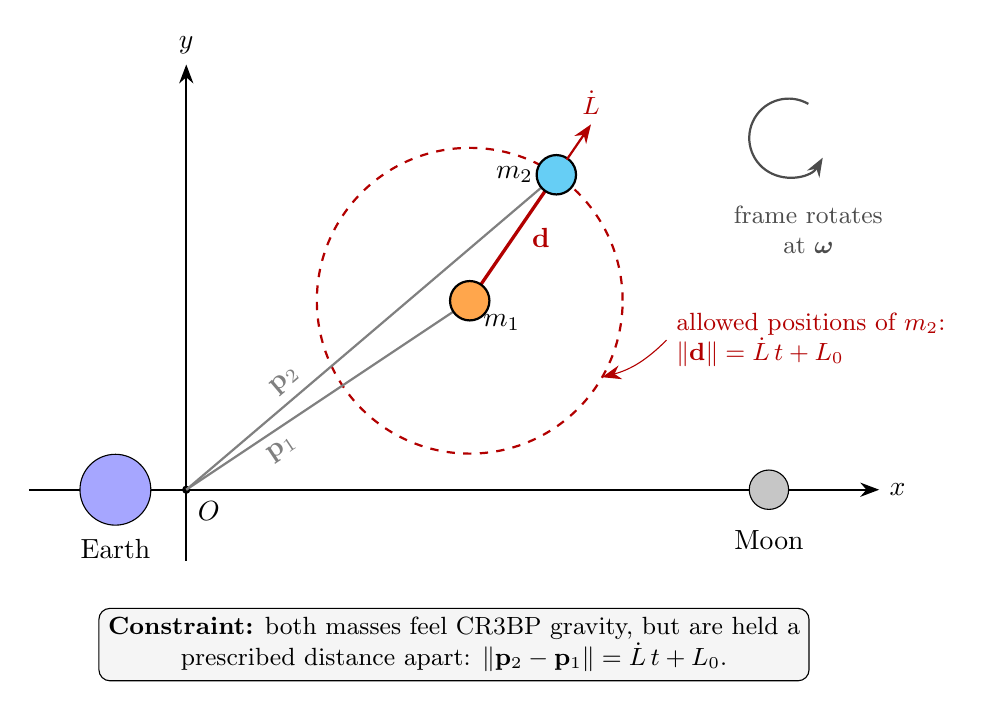
\begin{tikzpicture}[
    >={Stealth[length=2.4mm]},
    body/.style={circle, draw=black, thick, fill=#1, minimum size=5mm, inner sep=0pt},
    primary/.style={circle, draw=black, fill=#1, inner sep=0pt},
    posvec/.style={->, thick, gray},
]
    % Rotating CR3BP frame, centered on the Earth--Moon barycenter O (not to scale)
    \coordinate (O) at (0, 0);
    \coordinate (E) at (-0.9, 0);
    \coordinate (M) at (7.4, 0);
    \coordinate (P1) at (3.6, 2.4);
    \coordinate (P2) at (4.7, 4.0);

    % Axes, symmetric about the picture's horizontal center (x = 3.4)
    \draw[->, thick] (-2.0, 0) -- (8.8, 0) node[right] {$x$};
    \draw[->, thick] (0, -0.9) -- (0, 5.4) node[above] {$y$};
    \node[below right=1pt] at (O) {$O$};
    \fill (O) circle (1.5pt);

    % Earth and Moon (fixed in this frame)
    \node[primary=blue!35, minimum size=9mm] at (E) {};
    \node[below=5mm] at (E) {Earth};
    \node[primary=gray!45, minimum size=5mm] at (M) {};
    \node[below=4mm] at (M) {Moon};

    % Rotation of the frame, shown well away from the masses
    \draw[->, thick, black!70] (7.9, 4.9) arc (60:330:0.5);
    \node[black!70, align=center, font=\small] at (7.9, 3.3)
        {frame rotates\\ at $\boldsymbol{\omega}$};

    % Constraint circle: every position the second mass may occupy
    \pgfmathsetmacro{\rad}{sqrt((4.7-3.6)^2 + (4.0-2.4)^2)}
    \draw[dashed, thick, red!70!black] (P1) circle (\rad);
    \node[red!70!black, align=left, font=\small, anchor=west] (circlelabel)
        at (6.1, 1.9) {allowed positions of $m_2$:\\ $\lVert\mathbf{d}\rVert = \dot{L}\,t + L_0$};
    \draw[red!70!black, ->] (circlelabel.west) to[bend left=15]
        ($(P1) + (-30:\rad)$);

    % Position vectors from the origin, labeled along their length
    \draw[posvec] (O) -- (P1) node[pos=0.3, below, sloped] {$\mathbf{p}_1$};
    \draw[posvec] (O) -- (P2) node[pos=0.3, above, sloped] {$\mathbf{p}_2$};

    % Separation vector
    \draw[->, very thick, red!70!black] (P1) -- (P2)
        node[midway, right=3pt] {$\mathbf{d}$};

    % Masses; labels sit on the side away from the circle and the vectors
    \node[body=orange!70] at (P1) {};
    \node[below right=2pt] at (P1) {$m_1$};
    \node[body=cyan!60] at (P2) {};
    \node[left=5pt] at (P2) {$m_2$};

    % Rate of change of the radius
    \draw[->, thick, red!70!black] ($(P1)!1.12!(P2)$) -- ($(P1)!1.4!(P2)$)
        node[above, font=\small] {$\dot{L}$};

    % Plain-language statement of the constraint, centered under the diagram
    \node[draw, rounded corners, fill=gray!8, align=center, font=\small,
          anchor=north] at (3.4, -1.5)
        {\textbf{Constraint:} both masses feel CR3BP gravity, but are held a\\
         prescribed distance apart: $\lVert\mathbf{p}_2 - \mathbf{p}_1\rVert = \dot{L}\,t + L_0$.};
\end{tikzpicture}
\caption{Two point masses $m_1$ and $m_2$ in the rotating CR3BP frame (schematic, not
to scale). Gravity from the Earth and Moon acts on each mass, but the separation
$\mathbf{d} = \mathbf{p}_2 - \mathbf{p}_1$ is forced to equal $\dot{L}t + L_0$: $m_2$ must lie on the dashed
circle about $m_1$, whose radius changes at the rate $\dot{L}$.}
\label{fig:setup}
\end{figure}

This note derives the equations of motion for two point masses, $m_1$ and $m_2$, moving in the circular restricted three-body problem (CR3BP) while subject to a prescribed, possibly time-varying, constraint on their separation (for example, a tether of length $\dot{L} t + L_0$).  It then derives the Jacobian of the resulting dynamics, as needed for state transition matrix propagation.

The derivation proceeds in three steps:
\begin{enumerate}
    \item Section~\ref{sec:setup} defines the Lagrangian, the specific energies, and the constraint.
    \item Section~\ref{sec:eoms} applies the Euler--Lagrange equations with a Lagrange multiplier and eliminates the multiplier to obtain closed-form constrained accelerations.
    \item Section~\ref{sec:jacobian} differentiates those accelerations with respect to the state.
\end{enumerate}

\section{System Setup}
\label{sec:setup}

\subsection{Lagrangian and energies}

The positions $\mathbf{p}_i$ are expressed in the rotating CR3BP frame, which has angular velocity $\boldsymbol{\omega}$.  The Earth and Moon (the primary and secondary) are fixed in this frame at $\mathbf{r}_E$ and $\mathbf{r}_M$, and $\mu$ is the CR3BP mass parameter.  The Lagrangian of the system, $\mathcal{L}$, is the difference between the kinetic and potential energies:

\begin{equation*}
	\mathcal{L} = T - V = T_1(\mathbf{p}_1, \dot{\mathbf{p}}_1) + T_2(\mathbf{p}_2, \dot{\mathbf{p}}_2) - V_1(\mathbf{p}_1) - V_2(\mathbf{p}_2)
\end{equation*}

The kinetic terms use the inertial velocity of each mass, written in the rotating frame, and the potential terms are the gravitational potentials of the two primaries:

\begin{align}
\begin{split}
    T_1 &= \frac{1}{2} m_1 \left(\dot{\mathbf{p}}_1 + \lfloor \boldsymbol{\omega} \rfloor_\times \mathbf{p}_1\right)^T \left(\dot{\mathbf{p}}_1 + \lfloor \boldsymbol{\omega} \rfloor_\times \mathbf{p}_1\right) \\
    T_2 &= \frac{1}{2} m_2 \left(\dot{\mathbf{p}}_2 + \lfloor \boldsymbol{\omega} \rfloor_\times \mathbf{p}_2\right)^T \left(\dot{\mathbf{p}}_2 + \lfloor \boldsymbol{\omega} \rfloor_\times \mathbf{p}_2\right) \\
    V_1 &= -m_1 \frac{1-\mu}{\norm{\mathbf{p}_1 - \mathbf{r}_E}} - m_1 \frac{\mu}{\norm{\mathbf{p}_1 - \mathbf{r}_M}} \\
    V_2 &= -m_2 \frac{1-\mu}{\norm{\mathbf{p}_2 - \mathbf{r}_E}} - m_2 \frac{\mu}{\norm{\mathbf{p}_2 - \mathbf{r}_M}}
\end{split}
\end{align}

Dividing all terms through by the total mass $M = m_1 + m_2$ yields specific (per-unit-mass) energies.  With the mass fraction $\eta = m_2 / M$ (so that $m_1 / M = 1 - \eta$), they become:


\begin{align}
\begin{split}
    T_1 &= \frac{1-\eta}{2} \left(\mathbf{v}_1 \cdot \mathbf{v}_1\right) \\
    T_2 &= \frac{\eta}{2} \left(\mathbf{v}_2 \cdot \mathbf{v}_2\right) \\
    V_1 &= -(1-\eta)(1-\mu) (\mathbf{e}_1 \cdot \mathbf{e}_1)^{-1/2} - (1-\eta)\mu (\mathbf{m}_1 \cdot \mathbf{m}_1)^{-1/2} \\
    V_2 &= -\eta(1-\mu) (\mathbf{e}_2 \cdot \mathbf{e}_2)^{-1/2} - \eta \mu (\mathbf{m}_2 \cdot \mathbf{m}_2)^{-1/2}
\end{split}
\end{align}

The auxiliary velocity and relative-position vectors are $\mathbf{v}_1 = \dot{\mathbf{p}}_1 + \lfloor \boldsymbol{\omega} \rfloor_\times \mathbf{p}_1$, $\mathbf{v}_2 = \dot{\mathbf{p}}_2 + \lfloor \boldsymbol{\omega} \rfloor_\times \mathbf{p}_2$, $\mathbf{e}_1 = \mathbf{p}_1 - \mathbf{r}_E$, $\mathbf{e}_2 = \mathbf{p}_2 - \mathbf{r}_E$, $\mathbf{m}_1 = \mathbf{p}_1 - \mathbf{r}_M$, and $\mathbf{m}_2 = \mathbf{p}_2 - \mathbf{r}_M$.

\subsection{Separation constraint}

The two masses are subject to a time-dependent holonomic constraint that fixes their separation, $\mathbf{d} = \mathbf{p}_2 - \mathbf{p}_1$, to the length $\dot{L} t + L_0$:

\begin{align}
\begin{split}
    g(\mathbf{p}_1, \mathbf{p}_2) &= (\mathbf{p}_2 - \mathbf{p}_1)^T(\mathbf{p}_2 - \mathbf{p}_1) - (\dot{L} t + L_0)^2 \\
    &= \mathbf{d}^T \mathbf{d} - (\dot{L} t + L_0)^2 = 0, \quad \mathbf{d} = \mathbf{p}_2 - \mathbf{p}_1
\end{split}
\end{align}

\section{Constrained Equations of Motion}
\label{sec:eoms}

\subsection{Euler--Lagrange equations with a multiplier}

Enforcing the constraint with a Lagrange multiplier $\lambda$, the Euler--Lagrange equations for the two masses are:

\begin{align}
\begin{split}
    \frac{d}{dt} \pd{\mathcal{L}}{\dot{\mathbf{p}}_1} - \pd{\mathcal{L}}{\mathbf{p}_1} &= \lambda \pd{g}{\mathbf{p}_1} \\
    \frac{d}{dt} \pd{\mathcal{L}}{\dot{\mathbf{p}}_2} - \pd{\mathcal{L}}{\mathbf{p}_2} &= \lambda \pd{g}{\mathbf{p}_2} \\
\end{split}
\end{align}

These are six scalar equations in seven unknowns ($\ddot{\mathbf{p}}_1$, $\ddot{\mathbf{p}}_2$, and $\lambda$), so one more equation is needed.  It is supplied by the constraint itself, which must hold at all times.  Differentiating the constraint twice turns it into an acceleration-level condition that can be solved together with the Euler--Lagrange equations:

\begin{equation}
    \frac{d^2 g(\mathbf{p}_1, \mathbf{p}_2)}{dt^2} = 2 (\dot{\mathbf{p}}_2 - \dot{\mathbf{p}}_1)^T(\dot{\mathbf{p}}_2 - \dot{\mathbf{p}}_1) + 2 (\mathbf{p}_2 - \mathbf{p}_1)^T(\ddot{\mathbf{p}}_2 - \ddot{\mathbf{p}}_1) - 2 \dot{L}^2 = 0
\end{equation}

\subsection{Unconstrained accelerations}

In the CR3BP, where $\boldsymbol{\omega} = \hat{\mathbf{z}}$ in nondimensional units, the momentum-rate term $\frac{d}{dt} \pd{\mathcal{L}}{\dot{\mathbf{p}}_i}$ has the form:

\begin{equation}
    \left[ \frac{d}{dt} \pd{\mathcal{L}}{\dot{\mathbf{p}}_i} \right]^T = \bar{m}_i \left( \begin{bmatrix}
        \ddot{x}_i \\ \ddot{y}_i \\ \ddot{z}_i
    \end{bmatrix} + \begin{bmatrix}
        0 \\ 0 \\ 1
    \end{bmatrix} \times \begin{bmatrix}
        \dot{x}_i \\ \dot{y}_i \\ \dot{z}_i
    \end{bmatrix} \right) = \bar{m}_i \left( \ddot{\mathbf{p}}_i + \boldsymbol{\omega} \times \dot{\mathbf{p}}_i \right)
\end{equation}

where $\bar{m}_1 = 1-\eta$ and $\bar{m}_2 = \eta$ are the normalized masses.  Substituting this into the Euler--Lagrange equations and moving the Coriolis terms to the right-hand side gives:

\begin{align}
\begin{split}
    (1-\eta) \ddot{\mathbf{p}}_1 - \lambda \pd{g}{\mathbf{p}_1} &= \pd{\mathcal{L}}{\mathbf{p}_1} - (1-\eta) \left(\boldsymbol{\omega} \times \dot{\mathbf{p}}_1\right) \\
    \eta \ddot{\mathbf{p}}_2 - \lambda \pd{g}{\mathbf{p}_2} &= \pd{\mathcal{L}}{\mathbf{p}_2} - \eta \left(\boldsymbol{\omega} \times \dot{\mathbf{p}}_2\right) \\
\end{split}
\end{align}

Without the constraint ($\lambda = 0$), these reduce to the standard equations of motion for each particle.  This defines the unconstrained accelerations $\mathbf{a}_1$ and $\mathbf{a}_2$ that each mass would have in the absence of the constraint:

\begin{align}
\begin{split}
    (1-\eta) \mathbf{a}_1 &= \pd{\mathcal{L}}{\mathbf{p}_1} - (1-\eta) \left(\boldsymbol{\omega} \times \dot{\mathbf{p}}_1\right) \\
    \eta \mathbf{a}_2 &= \pd{\mathcal{L}}{\mathbf{p}_2} - \eta \left(\boldsymbol{\omega} \times \dot{\mathbf{p}}_2\right) \\
\end{split}
\end{align}

Substituting these definitions into the right-hand sides of the constrained equations gives:

\begin{align}
\begin{split}
    (1-\eta) \ddot{\mathbf{p}}_1 - \lambda \pd{g}{\mathbf{p}_1} &= (1-\eta) \mathbf{a}_1 \\
    \eta \ddot{\mathbf{p}}_2 - \lambda \pd{g}{\mathbf{p}_2} &= \eta \mathbf{a}_2 \\
\end{split}
\end{align}

\subsection{Solving for the multiplier}

The acceleration-level constraint can be rewritten in terms of $\mathbf{d}$ and its derivatives:
\begin{equation}
    \frac{d^2 g(\mathbf{p}_1, \mathbf{p}_2)}{dt^2} = 2 \dot{\mathbf{d}}^T \dot{\mathbf{d}} + 2 \mathbf{d}^T (\ddot{\mathbf{p}}_2 - \ddot{\mathbf{p}}_1) - 2 \dot{L}^2 = 0
\end{equation}

Moving the acceleration terms to the left-hand side gives

\begin{equation}
    2 \mathbf{d}^T \ddot{\mathbf{p}}_2 - 2 \mathbf{d}^T \ddot{\mathbf{p}}_1 = 2 \dot{L}^2 - 2 \dot{\mathbf{d}}^T \dot{\mathbf{d}}
\end{equation}

The constraint gradients are $\pd{g}{\mathbf{p}_1} = -2 \mathbf{d}^T$ and $\pd{g}{\mathbf{p}_2} = 2 \mathbf{d}^T$.  Stacking the two constrained equations of motion with the acceleration-level constraint gives a single linear system in $\ddot{\mathbf{p}}_1$, $\ddot{\mathbf{p}}_2$, and $\lambda$, whose right-hand side contains only known quantities:

\begin{equation}
    \begin{bmatrix}
        (1-\eta) \mathbf{I}_3 & \mathbf{0}_3 & 2\mathbf{d} \\
        \mathbf{0}_3 & \eta \mathbf{I}_3 & -2\mathbf{d} \\
        -2\mathbf{d}^T & 2\mathbf{d}^T & 0
    \end{bmatrix} \begin{bmatrix}
        \ddot{\mathbf{p}}_1 \\
        \ddot{\mathbf{p}}_2 \\
        \lambda
    \end{bmatrix} = \begin{bmatrix}
        (1-\eta) \mathbf{a}_1 \\
        \eta \mathbf{a}_2 \\
        2 \dot{L}^2 - 2 \dot{\mathbf{d}}^T \dot{\mathbf{d}}
    \end{bmatrix}
\end{equation}

\subsection{Closed-form constrained accelerations}

Inverting this system expresses the constrained accelerations as a linear map of the unconstrained accelerations plus a velocity-dependent correction:

\begin{equation}
    \begin{bmatrix}
        \ddot{\mathbf{p}}_1 \\
        \ddot{\mathbf{p}}_2
    \end{bmatrix} = \begin{bmatrix}
        \mathbf{I}_3 - \eta \mathbf{D} & \eta \mathbf{D} \\
        (1-\eta) \mathbf{D} & \mathbf{I}_3 - (1-\eta) \mathbf{D}
    \end{bmatrix} \begin{bmatrix}
        \mathbf{a}_1 \\
        \mathbf{a}_2 \end{bmatrix} + \begin{bmatrix}
            \eta \mathbf{q} \\
            -(1-\eta) \mathbf{q} \\
        \end{bmatrix}
\end{equation}

where $\mathbf{D} = (\mathbf{d} \mathbf{d}^T) / (\mathbf{d}^T \mathbf{d})$ is the projector onto the direction of $\mathbf{d}$, and the correction vector is

\begin{equation}
    \mathbf{q} = \frac{\dot{\mathbf{d}}^T \dot{\mathbf{d}} - \dot{L}^2}{\mathbf{d}^T \mathbf{d}} \mathbf{d}
\end{equation}

\section{Jacobian of the Dynamics}
\label{sec:jacobian}

\subsection{Structure of the constrained accelerations}

Expanding the block form from the previous section, the constrained accelerations are:

\begin{align}
\begin{split}
    \ddot{\mathbf{p}}_1 &= \mathbf{a}_1 + \eta \left[ \mathbf{D} (\mathbf{a}_2 - \mathbf{a}_1) + \mathbf{q} \right] \\
    \ddot{\mathbf{p}}_2 &= \mathbf{a}_2 - (1-\eta) \left[ \mathbf{D} (\mathbf{a}_2 - \mathbf{a}_1) + \mathbf{q} \right]
\end{split}
\end{align}

The term $\mathbf{D} (\mathbf{a}_2 - \mathbf{a}_1) + \mathbf{q}$ appears in both equations, scaled by $\eta$ and $-(1-\eta)$ respectively.  Its partial derivatives with respect to the positions and velocities therefore need to be computed only once and are shared by $\ddot{\mathbf{p}}_1$ and $\ddot{\mathbf{p}}_2$.  We examine its two pieces in turn, beginning with the first:

\begin{equation}
    \mathbf{D} (\mathbf{a}_2 - \mathbf{a}_1) = \frac{\mathbf{d}^T (\mathbf{a}_2 - \mathbf{a}_1)}{\mathbf{d}^T \mathbf{d}} \mathbf{d}
\end{equation}

The second piece is $\mathbf{q}$, which was defined above as:

\begin{equation}
    \mathbf{q} = \frac{\dot{\mathbf{d}}^T \dot{\mathbf{d}} - \dot{L}^2}{\mathbf{d}^T \mathbf{d}} \mathbf{d}
\end{equation}

Both pieces are proportional to $\mathbf{d}$ and share the factor $(\mathbf{d}^T \mathbf{d})^{-1}$, so they can be differentiated with the same technique.  The full term can be split into the individual contributions of $\mathbf{a}_1$, $\mathbf{a}_2$, and $\mathbf{q}$:

\begin{equation}
    \mathbf{D} (\mathbf{a}_2 - \mathbf{a}_1) + \mathbf{q} = \mathbf{D} \mathbf{a}_2 - \mathbf{D} \mathbf{a}_1 + \mathbf{q}
\end{equation}

\begin{equation}
    \mathbf{D} \mathbf{a}_i = \frac{\mathbf{d} \mathbf{d}^T}{\mathbf{d}^T \mathbf{d}} \mathbf{a}_i = (\mathbf{d} \cdot \mathbf{a}_i) (\mathbf{d} \cdot \mathbf{d})^{-1} \mathbf{d}
\end{equation}

\subsection{Derivatives of $\mathbf{D} \mathbf{a}_i$}

The product $\mathbf{D} \mathbf{a}_i$ is a scalar numerator $(\mathbf{d} \cdot \mathbf{a}_i)$, a scalar $(\mathbf{d} \cdot \mathbf{d})^{-1}$, and the vector $\mathbf{d}$.  Differentiating it with respect to $\mathbf{p}_j$ requires the product rule and the derivatives of the two scalar factors:

\begin{equation}
    \pd{(\mathbf{d} \cdot \mathbf{a}_i)}{\mathbf{p}_j} = \mathbf{a}_i^T \pd{\mathbf{d}}{\mathbf{p}_j} + \mathbf{d}^T \pd{\mathbf{a}_i}{\mathbf{p}_j}
\end{equation}

\begin{equation}
    \pd{(\mathbf{d} \cdot \mathbf{d})^{-1}}{\mathbf{p}_j} = -\frac{2}{(\mathbf{d} \cdot \mathbf{d})^2} \mathbf{d}^T \pd{\mathbf{d}}{\mathbf{p}_j}
\end{equation}

Combining these with the product rule gives the general position derivative:

\begin{align}
\begin{split}
    \pd{\mathbf{D} \mathbf{a}_i}{\mathbf{p}_j}
    &= \pddown{(\mathbf{d} \cdot \mathbf{a}_i) (\mathbf{d} \cdot \mathbf{d})^{-1} \mathbf{d}}{\mathbf{p}_j} \\
    &= (\mathbf{d} \cdot \mathbf{d})^{-1} \mathbf{d} \pd{(\mathbf{d} \cdot \mathbf{a}_i)}{\mathbf{p}_j} + (\mathbf{d} \cdot \mathbf{a}_i) \mathbf{d} \pd{(\mathbf{d} \cdot \mathbf{d})^{-1}}{\mathbf{p}_j} + \frac{\mathbf{d}\cdot\mathbf{a}_i}{\mathbf{d} \cdot \mathbf{d}} \pd{\mathbf{d}}{\mathbf{p}_j} \\
    &= (\mathbf{d} \cdot \mathbf{d})^{-1} \mathbf{d} \left[ \mathbf{a}_i^T \pd{\mathbf{d}}{\mathbf{p}_j} + \mathbf{d}^T \pd{\mathbf{a}_i}{\mathbf{p}_j} \right] + (\mathbf{d} \cdot \mathbf{a}_i) \mathbf{d} \left[ -\frac{2}{(\mathbf{d} \cdot \mathbf{d})^2} \mathbf{d}^T \pd{\mathbf{d}}{\mathbf{p}_j} \right] + \frac{\mathbf{d}\cdot\mathbf{a}_i}{\mathbf{d} \cdot \mathbf{d}} \pd{\mathbf{d}}{\mathbf{p}_j} \\
    &= \mathbf{D} \pd{\mathbf{a}_i}{\mathbf{p}_j} + \frac{1}{\mathbf{d} \cdot \mathbf{d}} \left[ \mathbf{d} \mathbf{a}_i^T + (\mathbf{d}\cdot\mathbf{a}_i) (\mathbf{I} - 2 \mathbf{D}) \right] \pd{\mathbf{d}}{\mathbf{p}_j} \\
\end{split}
\end{align}

Since $\pd{\mathbf{d}}{\mathbf{p}_1} = -\mathbf{I}$ and $\pd{\mathbf{d}}{\mathbf{p}_2} = \mathbf{I}$, specializing to each pair of masses gives the position derivatives:

\begin{align}
\begin{split}
    \pd{\mathbf{D} \mathbf{a}_1}{\mathbf{p}_1} &= \mathbf{D} \pd{\mathbf{a}_1}{\mathbf{p}_1} - \frac{1}{\mathbf{d} \cdot \mathbf{d}} \left[ \mathbf{d} \mathbf{a}_1^T + (\mathbf{d}\cdot\mathbf{a}_1) (\mathbf{I} - 2 \mathbf{D}) \right] \\
    \pd{\mathbf{D} \mathbf{a}_1}{\mathbf{p}_2} &= \frac{1}{\mathbf{d} \cdot \mathbf{d}} \left[ \mathbf{d} \mathbf{a}_1^T + (\mathbf{d}\cdot\mathbf{a}_1) (\mathbf{I} - 2 \mathbf{D}) \right] \\
    \pd{\mathbf{D} \mathbf{a}_2}{\mathbf{p}_1} &= -\frac{1}{\mathbf{d} \cdot \mathbf{d}} \left[ \mathbf{d} \mathbf{a}_2^T + (\mathbf{d}\cdot\mathbf{a}_2) (\mathbf{I} - 2 \mathbf{D}) \right] \\
    \pd{\mathbf{D} \mathbf{a}_2}{\mathbf{p}_2} &= \mathbf{D} \pd{\mathbf{a}_2}{\mathbf{p}_2} + \frac{1}{\mathbf{d} \cdot \mathbf{d}} \left[ \mathbf{d} \mathbf{a}_2^T + (\mathbf{d}\cdot\mathbf{a}_2) (\mathbf{I} - 2 \mathbf{D}) \right] \\
\end{split}
\end{align}

The projector $\mathbf{D}$ depends only on positions, so the velocity derivatives involve only the acceleration Jacobians:

\begin{align}
\begin{split}
    \pd{\mathbf{D} \mathbf{a}_1}{\dot{\mathbf{p}}_1} &= \mathbf{D} \pd{\mathbf{a}_1}{\dot{\mathbf{p}}_1} \\
    \pd{\mathbf{D} \mathbf{a}_1}{\dot{\mathbf{p}}_2} &= \mathbf{0} \\
    \pd{\mathbf{D} \mathbf{a}_2}{\dot{\mathbf{p}}_1} &= \mathbf{0} \\
    \pd{\mathbf{D} \mathbf{a}_2}{\dot{\mathbf{p}}_2} &= \mathbf{D} \pd{\mathbf{a}_2}{\dot{\mathbf{p}}_2} \\
\end{split}
\end{align}

\subsection{Derivatives of $\mathbf{q}$}

The correction vector can be written as:

\begin{equation}
    \mathbf{q} = (\dot{\mathbf{d}} \cdot \dot{\mathbf{d}} - \dot{L}^2) (\mathbf{d} \cdot \mathbf{d})^{-1} \mathbf{d}
\end{equation}

Its derivative with respect to a general position $\mathbf{p}_i$ is:

\begin{align}
\begin{split}
    \pd{\mathbf{q}}{\mathbf{p}_i}
    &= \pddown{(\dot{\mathbf{d}} \cdot \dot{\mathbf{d}} - \dot{L}^2) (\mathbf{d} \cdot \mathbf{d})^{-1} \mathbf{d}}{\mathbf{p}_i} \\
    &= (\dot{\mathbf{d}} \cdot \dot{\mathbf{d}} - \dot{L}^2) \pddown{(\mathbf{d} \cdot \mathbf{d})^{-1} \mathbf{d}}{\mathbf{p}_i} \\
    &= (\dot{\mathbf{d}} \cdot \dot{\mathbf{d}} - \dot{L}^2) \pddown{(\mathbf{d} \cdot \mathbf{d})^{-1} \mathbf{d}}{\mathbf{d}} \pd{\mathbf{d}}{\mathbf{p}_i} \\
    &= (\dot{\mathbf{d}} \cdot \dot{\mathbf{d}} - \dot{L}^2) \left[ \mathbf{d} \pd{(\mathbf{d} \cdot \mathbf{d})^{-1}}{\mathbf{d}} + \frac{1}{\mathbf{d} \cdot \mathbf{d}} \mathbf{I} \right] \pd{\mathbf{d}}{\mathbf{p}_i} \\
    &= \frac{\dot{\mathbf{d}} \cdot \dot{\mathbf{d}} - \dot{L}^2}{\mathbf{d} \cdot \mathbf{d}} \left[ \mathbf{I} - 2\mathbf{D} \right] \pd{\mathbf{d}}{\mathbf{p}_i} \\
\end{split}
\end{align}

Specializing to each mass gives:

\begin{align}
\begin{split}
    \pd{\mathbf{q}}{\mathbf{p}_1} &= -\frac{\dot{\mathbf{d}} \cdot \dot{\mathbf{d}} - \dot{L}^2}{\mathbf{d} \cdot \mathbf{d}} \left[ \mathbf{I} - 2\mathbf{D} \right] \\
    \pd{\mathbf{q}}{\mathbf{p}_2} &= +\frac{\dot{\mathbf{d}} \cdot \dot{\mathbf{d}} - \dot{L}^2}{\mathbf{d} \cdot \mathbf{d}} \left[ \mathbf{I} - 2\mathbf{D} \right] \\
\end{split}
\end{align}

The derivative with respect to a general velocity $\dot{\mathbf{p}}_i$ is simpler, because $\mathbf{d}$ does not depend on velocity:

\begin{align}
\begin{split}
    \pd{\mathbf{q}}{\dot{\mathbf{p}}_i}
    &= \pddown{(\dot{\mathbf{d}} \cdot \dot{\mathbf{d}} - \dot{L}^2) (\mathbf{d} \cdot \mathbf{d})^{-1} \mathbf{d}}{\dot{\mathbf{p}}_i} \\
    &= \frac{1}{\mathbf{d} \cdot \mathbf{d}} \mathbf{d} \pddown{\dot{\mathbf{d}} \cdot \dot{\mathbf{d}} - \dot{L}^2}{\dot{\mathbf{p}}_i} \\
    &= \frac{2}{\mathbf{d} \cdot \mathbf{d}} \mathbf{d} \dot{\mathbf{d}}^T \pd{\dot{\mathbf{d}}}{\dot{\mathbf{p}}_i} \\
\end{split}
\end{align}

Specializing to each mass gives:

\begin{align}
\begin{split}
    \pd{\mathbf{q}}{\dot{\mathbf{p}}_1} &= -\frac{2}{\mathbf{d} \cdot \mathbf{d}} \mathbf{d} \dot{\mathbf{d}}^T \\
    \pd{\mathbf{q}}{\dot{\mathbf{p}}_2} &= +\frac{2}{\mathbf{d} \cdot \mathbf{d}} \mathbf{d} \dot{\mathbf{d}}^T \\
\end{split}
\end{align}

Finally, for later use, the derivative of $\mathbf{q}$ with respect to the constraint rate $\dot{L}$ is:

\begin{align}
\begin{split}
    \pd{\mathbf{q}}{\dot{L}}
    &= \pddown{(\dot{\mathbf{d}} \cdot \dot{\mathbf{d}} - \dot{L}^2) (\mathbf{d} \cdot \mathbf{d})^{-1} \mathbf{d}}{\dot{L}} \\
    &= -\frac{2 \dot{L}}{\mathbf{d} \cdot \mathbf{d}} \mathbf{d} \\
\end{split}
\end{align}

\clearpage
\subsection{Summary of the partial derivatives}

\begin{align}
\begin{split}
    \ddot{\mathbf{p}}_1 &= \mathbf{a}_1 + \eta \left[ \mathbf{D} (\mathbf{a}_2 - \mathbf{a}_1) + \mathbf{q} \right] \\
    \ddot{\mathbf{p}}_2 &= \mathbf{a}_2 - (1-\eta) \left[ \mathbf{D} (\mathbf{a}_2 - \mathbf{a}_1) + \mathbf{q} \right]
\end{split}
\end{align}

Table~\ref{tab:jacobian} lists the partial derivatives of the constrained accelerations with respect to each state quantity, expressed in terms of the building blocks defined below.  The accelerations are repeated here for reference, and the table follows them:

\begin{table}[h]
    \centering
    \caption{Listing of all partial derivatives of the accelerations with respect to state quantities}
    \label{tab:jacobian}
    \resizebox{\textwidth}{!}{%
    \begin{tabular}{|l|c|c|c|c|}
        \hline
        & $\mathbf{p}_1$ & $\mathbf{p}_2$ & $\dot{\mathbf{p}}_1$ & $\dot{\mathbf{p}}_2$ \\
        \hline
        $\ddot{\mathbf{p}}_1$ & $\pd{\mathbf{a}_1}{\mathbf{p}_1} + \eta \left[ \pd{\mathbf{D} \mathbf{a}_2}{\mathbf{p}_1} - \pd{\mathbf{D} \mathbf{a}_1}{\mathbf{p}_1} + \pd{\mathbf{q}}{\mathbf{p}_1} \right]$ & $\eta \left[ \pd{\mathbf{D} \mathbf{a}_2}{\mathbf{p}_2} - \pd{\mathbf{D} \mathbf{a}_1}{\mathbf{p}_2} + \pd{\mathbf{q}}{\mathbf{p}_2} \right]$ & $\pd{\mathbf{a}_1}{\dot{\mathbf{p}}_1} + \eta \left[ \pd{\mathbf{q}}{\dot{\mathbf{p}}_1} - \mathbf{D} \pd{\mathbf{a}_1}{\dot{\mathbf{p}}_1} \right]$ & $\eta \left[ \pd{\mathbf{q}}{\dot{\mathbf{p}}_2} + \mathbf{D} \pd{\mathbf{a}_2}{\dot{\mathbf{p}}_2} \right]$ \\
        \hline
        $\ddot{\mathbf{p}}_2$ & $-(1-\eta) \left[ \pd{\mathbf{D} \mathbf{a}_2}{\mathbf{p}_1} - \pd{\mathbf{D} \mathbf{a}_1}{\mathbf{p}_1} + \pd{\mathbf{q}}{\mathbf{p}_1} \right]$ & $\pd{\mathbf{a}_2}{\mathbf{p}_2} - (1-\eta) \left[ \pd{\mathbf{D} \mathbf{a}_2}{\mathbf{p}_2} - \pd{\mathbf{D} \mathbf{a}_1}{\mathbf{p}_2} + \pd{\mathbf{q}}{\mathbf{p}_2} \right]$ & $-(1-\eta) \left[ \pd{\mathbf{q}}{\dot{\mathbf{p}}_1} - \mathbf{D} \pd{\mathbf{a}_1}{\dot{\mathbf{p}}_1} \right]$ & $\pd{\mathbf{a}_2}{\dot{\mathbf{p}}_2} - (1-\eta) \left[ \pd{\mathbf{q}}{\dot{\mathbf{p}}_2} + \mathbf{D} \pd{\mathbf{a}_2}{\dot{\mathbf{p}}_2} \right]$ \\
        \hline
    \end{tabular}
    }%
\end{table}

The building blocks are the derivatives of $\mathbf{D} \mathbf{a}_i$, the derivatives of $\mathbf{q}$, and the auxiliary terms $\mathbf{T}_1$ through $\mathbf{T}_4$, $\mathbf{D}$, and $\kappa$ defined at the end of this subsection.  The derivatives of $\mathbf{D} \mathbf{a}_i$ are:

\begin{equation*}
    \pd{\mathbf{D} \mathbf{a}_1}{\mathbf{p}_1} = \mathbf{D} \pd{\mathbf{a}_1}{\mathbf{p}_1} - \mathbf{T}_1 - \mathbf{T}_2
\end{equation*}

\begin{equation*}
    \pd{\mathbf{D} \mathbf{a}_1}{\mathbf{p}_2} = \mathbf{T}_1 + \mathbf{T}_2
\end{equation*}

\begin{equation*}
    \pd{\mathbf{D} \mathbf{a}_2}{\mathbf{p}_1} = -\mathbf{T}_3 - \mathbf{T}_4
\end{equation*}

\begin{equation*}
    \pd{\mathbf{D} \mathbf{a}_2}{\mathbf{p}_2} = \mathbf{D} \pd{\mathbf{a}_2}{\mathbf{p}_2} + \mathbf{T}_3 + \mathbf{T}_4
\end{equation*}

\begin{equation*}
    \pd{\mathbf{D} \mathbf{a}_1}{\dot{\mathbf{p}}_1} = \mathbf{D} \pd{\mathbf{a}_1}{\dot{\mathbf{p}}_1}
\end{equation*}

\begin{equation*}
    \pd{\mathbf{D} \mathbf{a}_2}{\dot{\mathbf{p}}_2} = \mathbf{D} \pd{\mathbf{a}_2}{\dot{\mathbf{p}}_2}
\end{equation*}

The derivatives of $\mathbf{q}$ are:

\begin{equation}
    \pd{\mathbf{q}}{\mathbf{p}_1} = -\frac{\kappa}{\mathbf{d} \cdot \mathbf{d}} \left[ \mathbf{I} - 2\mathbf{D} \right]
\end{equation}

\begin{equation}
    \pd{\mathbf{q}}{\mathbf{p}_2} = \frac{\kappa}{\mathbf{d} \cdot \mathbf{d}} \left[ \mathbf{I} - 2\mathbf{D} \right]
\end{equation}

\begin{equation}
    \pd{\mathbf{q}}{\dot{\mathbf{p}}_1} = -\frac{2}{\mathbf{d} \cdot \mathbf{d}} (\mathbf{d} \dot{\mathbf{d}}^T)
\end{equation}

\begin{equation}
    \pd{\mathbf{q}}{\dot{\mathbf{p}}_2} = \frac{2}{\mathbf{d} \cdot \mathbf{d}} (\mathbf{d} \dot{\mathbf{d}}^T)
\end{equation}

The auxiliary terms used above are defined as:

\begin{equation*}
    \mathbf{T}_1 = \frac{1}{\mathbf{d} \cdot \mathbf{d}} (\mathbf{d} \mathbf{a}_1^T), \quad\quad \mathbf{T}_2 = \frac{\mathbf{d}\cdot\mathbf{a}_1}{\mathbf{d} \cdot \mathbf{d}} (\mathbf{I} - 2 \mathbf{D})
\end{equation*}

\begin{equation*}
    \mathbf{T}_3 = \frac{1}{\mathbf{d} \cdot \mathbf{d}} (\mathbf{d} \mathbf{a}_2^T), \quad\quad \mathbf{T}_4 = \frac{\mathbf{d}\cdot\mathbf{a}_2}{\mathbf{d} \cdot \mathbf{d}} (\mathbf{I} - 2 \mathbf{D})
\end{equation*}

\begin{equation*}
    \mathbf{D} = \frac{\mathbf{d} \mathbf{d}^T}{\mathbf{d} \cdot \mathbf{d}}
\end{equation*}

\begin{equation*}
    \kappa = \dot{\mathbf{d}} \cdot \dot{\mathbf{d}} - \dot{L}^2
\end{equation*}

\subsection{Grouped form of the Jacobian}

The terms can be grouped by the external Jacobian ($\pd{\mathbf{a}_i}{\mathbf{p}_i}$ or $\pd{\mathbf{a}_i}{\dot{\mathbf{p}}_i}$) they multiply.  Defining

\begin{equation*}
    \mathbf{S} = \mathbf{T}_3 + \mathbf{T}_4 - \mathbf{T}_1 - \mathbf{T}_2
    = \frac{1}{\mathbf{d} \cdot \mathbf{d}} \left[ \mathbf{d} (\mathbf{a}_2 - \mathbf{a}_1)^T + \left(\mathbf{d} \cdot (\mathbf{a}_2 - \mathbf{a}_1)\right) (\mathbf{I} - 2\mathbf{D}) \right]
\end{equation*}

\begin{equation*}
    \mathbf{K} = \frac{\kappa}{\mathbf{d} \cdot \mathbf{d}} \left[ \mathbf{I} - 2\mathbf{D} \right], \quad\quad
    \mathbf{W} = \frac{2}{\mathbf{d} \cdot \mathbf{d}} (\mathbf{d} \dot{\mathbf{d}}^T)
\end{equation*}

so that $\pd{\mathbf{q}}{\mathbf{p}_1} = -\mathbf{K}$, $\pd{\mathbf{q}}{\mathbf{p}_2} = \mathbf{K}$, $\pd{\mathbf{q}}{\dot{\mathbf{p}}_1} = -\mathbf{W}$, and $\pd{\mathbf{q}}{\dot{\mathbf{p}}_2} = \mathbf{W}$, the eight blocks of the Jacobian are given in Table~\ref{tab:jacobian_grouped}.

\begin{table}[h]
    \centering
    \caption{Jacobian blocks grouped by external Jacobian components}
    \label{tab:jacobian_grouped}
    \resizebox{\textwidth}{!}{%
    \renewcommand{\arraystretch}{2.2}%
    \begin{tabular}{|l|c|c|c|c|}
        \hline
        & $\mathbf{p}_1$ & $\mathbf{p}_2$ & $\dot{\mathbf{p}}_1$ & $\dot{\mathbf{p}}_2$ \\
        \hline
        $\ddot{\mathbf{p}}_1$ & $\left( \mathbf{I} - \eta \mathbf{D} \right) \pd{\mathbf{a}_1}{\mathbf{p}_1} - \eta \left( \mathbf{S} + \mathbf{K} \right)$ & $\eta \mathbf{D} \pd{\mathbf{a}_2}{\mathbf{p}_2} + \eta \left( \mathbf{S} + \mathbf{K} \right)$ & $\left( \mathbf{I} - \eta \mathbf{D} \right) \pd{\mathbf{a}_1}{\dot{\mathbf{p}}_1} - \eta \mathbf{W}$ & $\eta \mathbf{D} \pd{\mathbf{a}_2}{\dot{\mathbf{p}}_2} + \eta \mathbf{W}$ \\
        \hline
        $\ddot{\mathbf{p}}_2$ & $(1-\eta) \mathbf{D} \pd{\mathbf{a}_1}{\mathbf{p}_1} + (1-\eta) \left( \mathbf{S} + \mathbf{K} \right)$ & $\left( \mathbf{I} - (1-\eta) \mathbf{D} \right) \pd{\mathbf{a}_2}{\mathbf{p}_2} - (1-\eta) \left( \mathbf{S} + \mathbf{K} \right)$ & $(1-\eta) \mathbf{D} \pd{\mathbf{a}_1}{\dot{\mathbf{p}}_1} + (1-\eta) \mathbf{W}$ & $\left( \mathbf{I} - (1-\eta) \mathbf{D} \right) \pd{\mathbf{a}_2}{\dot{\mathbf{p}}_2} - (1-\eta) \mathbf{W}$ \\
        \hline
    \end{tabular}%
    }
\end{table}

As a consistency check, the coefficients multiplying the external Jacobians reproduce the block matrix $\begin{bmatrix} \mathbf{I}_3 - \eta \mathbf{D} & \eta \mathbf{D} \\ (1-\eta) \mathbf{D} & \mathbf{I}_3 - (1-\eta) \mathbf{D} \end{bmatrix}$ from the inverted system, as expected.

\end{document}
